\documentclass[
  11pt,
  letterpaper,
   addpoints,
  answers
  ]{exam}

% Carga el preámbulo localizado en la carpeta superior
\NeedsTeXFormat{LaTeX2e}[2023/04/30]

% Provide the name of your page, the date it was last updated, and a comment about what it's used for
\ProvidesPackage{../exercise-preamble}[2023/04/30 Prof. Cassanelli custom LaTeX style]

% \usepackage{printlen}
% \uselengthunit{in}\printlength{\textwidth}

% PACKAGES
\usepackage[dvipsnames]{xcolor}

\usepackage{graphicx}
\graphicspath{{../figures}}
\usepackage{amsmath,amsthm,amssymb,mathtools,mathrsfs}
\usepackage{commath}
\usepackage{upgreek}
\usepackage{cancel}
\usepackage{enumerate}
\usepackage[font=small]{caption}
\usepackage[normalem]{ulem}
\usepackage{steinmetz}
\usepackage{enumitem}
\usepackage[left=1.5cm, right=1.5cm, top=1cm]{geometry}
\usepackage{wrapfig}

% REFERENCES AND OTHERS
\usepackage{../aas_macros}
\usepackage{natbib}
\bibpunct{(}{)}{;}{a}{}{,}

\usepackage{tikz}
\usepackage{tikz-3dplot}
\usepackage{circuitikz}
\usepackage{pgfplots}
\pgfplotsset{compat=1.15}
\usepgfplotslibrary{smithchart}
\usetikzlibrary{
  decorations.pathmorphing,
  decorations.markings,
  calc,
  patterns,
  decorations,
  angles,
  quotes,
  ext.topaths.arcthrough,
  shapes
  }

\usepackage{siunitx}
\sisetup{
    range-phrase=\text{--},
    range-units=single,
    separate-uncertainty=true,
    print-unity-mantissa=false
    }
\DeclareSIUnit{\gauss}{G}
\DeclareSIUnit{\jansky}{Jy}

\newcommand{\iu}{\mathrm{i}\mkern1mu}
\newcommand{\ju}{\mathrm{j}\mkern1mu}
\newcommand{\euler}{\mathrm{e}}
\newcommand{\exponential}[1]{\mathrm{exp}\left[#1\right]}
\newcommand{\uvec}[1]{\widehat{\mathbf{#1}}}
\newcommand{\uvecs}[1]{\boldsymbol{\widehat{#1}}}
\newcommand{\bvec}[1]{\boldsymbol{\mathcal{#1}}}

\usepackage{hyperref}
\hypersetup{
    % bookmarks=true,
    unicode=true,
    pdftoolbar=true,
    pdfmenubar=true,
    pdffitwindow=false,
    pdfstartview={FitH},
    pdftitle={EL3103},
    pdfauthor={Tomas Cassanelli},
    pdfcreator={Tomas Cassanelli},
    pdfnewwindow=true,
    colorlinks=true,
    linkcolor=Violet,
    citecolor=Violet,
    urlcolor=Violet
    }

% Exam document class
\renewcommand{\figurename}{Figura}
\renewcommand{\tablename}{Cuadro}
\pagestyle{empty}

\usepackage[spanish]{cleveref}

\crefname{question}{\protect{pregunta}}{\protect{preguntas}}
\Crefname{question}{\protect{Pregunta}}{\protect{Preguntas}}
\creflabelformat{question}{#2{#1}#3}

\renewcommand{\solutiontitle}{\noindent\textbf{Solución:}\par\noindent}
\bracketedpoints
\pointname{~puntos}

\endinput

% Paquetes locales
\usepackage{float}
\usepackage{booktabs} % para \toprule, \midrule, \bottomrule
\usepackage{xcolor} % para colores

% Macros locales
\newcommand{\Rel}{\mathfrak{R}} % símbolo para la reluctancia

\begin{document}

% Numeración de página
\pagestyle{plain}
\pagenumbering{arabic}

\noindent
\begin{minipage}{0.47\textwidth}

\includegraphics[width=\textwidth]{../fcfm_die}
\end{minipage}
\begin{minipage}{0.53\textwidth}
\begin{center} 
\large\textbf{Análisis de Sistemas Dinámicos y Estimación} (EL3204-1) \\
\large\textbf{Clase auxiliar 5} \\
\normalsize Prof.~ Marcos Orchard - Sebastián Espinosa.\\
\normalsize Prof.~Aux.~Erik Sáez
\end{center}
\end{minipage}

\vspace{0.5cm}
\noindent
\vspace{.85cm}

\begin{questions}
%----------------------------
  \question Considere un sistema modelado por la siguiente ecuación de diferencias
\begin{equation}
y(k+2) + 4y(k+1) + 4y(k) = u(k).
\end{equation}

\begin{enumerate}
    \item Formule el sistema en variables de estado.
    \item Obtenga la MTE del sistema, y encuentre las funciones base.
    \item Determine estabilidad BIBS y BIBO del sistema.
    \item Diseñe un controlador realimentado en el estado que ubique los polos en $-0.5$ y $0.5$. Diseñe un observador de Luenberger para este sistema controlado.
\end{enumerate}
%---------------------------
\begin{solution}

\subsection*{Resolución 1.1}

Nos encontramos ante un sistema discreto, por lo que es importante considerar ciertos aspectos particulares al trabajar con sus expresiones. Dado que la dinámica está descrita por una ecuación en diferencias, la formulación en variables de estado puede abordarse a partir de la función de transferencia, la cual nos permitirá obtener una representación conveniente del sistema. Para hallar dicha función de transferencia, debemos aplicar la transformada $Z$ (en lugar de la de Laplace, propia de sistemas continuos), ya que el sistema evoluciona en tiempo discreto. Aplicando la transformada $Z$ con condiciones iniciales nulas, obtenemos.
\begin{align}
  \mathcal{Z}\{x[n+k]\}
= z^{k} X(z) \;-\; \sum_{i=0}^{k-1} x[i]\, z^{\,k-1-i},
\qquad k\in \mathbb{Z}_{\ge 1}.
\end{align}
para condiciones iniciales nulas tenemos:
\begin{align}
  \mathcal{Z}\{x[n+k]\}
= z^{k} X(z).
\end{align}
Por lo tanto para nuestro caso particular, tenemos que:
\begin{align}
  \mathcal{Z}\{y(k+2) + 4y(k+1) + 4y(k) &= u(k)\} \\
z^{2}Y(z)+4zY(z)+4Y(z)&=U(z).
\end{align}
Por lo que, considerando que $H(z)=Y(z)/U(z)$, podemos ver que
\begin{align}
H(z)=\frac{1}{z^{2}+4z+4}.
\end{align}
Podemos ver que el polinomio del denominador se puede factorizar como $(z+2)^{2}$ de modo que
\begin{equation}
H(z)=\frac{1}{(z+2)^{2}},
\end{equation}
lo que indica que el sistema posee un polo en $-2$ de multiplicidad algebraica $2$. Para formular el sistema en variables de estado, es útil expresar la función de transferencia en fracciones parciales. Sin embargo, en el caso de polos repetidos, no es correcto escribir
\begin{equation}
H(z)=\frac{\alpha}{z+2}+\frac{\beta}{z+2},
\end{equation}
ya que ambos términos tendrían el mismo denominador y, por lo tanto, no reflejarían la presencia del polo doble. En su lugar, la descomposición adecuada para un polo repetido es de la forma
\begin{equation}
H(z)=\frac{\alpha}{(z+2)^{2}}+\frac{\beta}{z+2},
\end{equation}
donde podemos ver rápidamente que necesariamente se debe tener $\alpha=1$ y $\beta=0$. Luego, esto nos permite expresar la salida en $Z$ como
\begin{align}
Y(z) = \frac{1}{(z+2)^{2}}\,U(z)+\frac{0}{z+2}\,U(z) \nonumber = \begin{pmatrix}1 & 0\end{pmatrix}
        \begin{pmatrix}
        \dfrac{U(z)}{(z+2)^{2}}\\[6pt]
        \dfrac{U(z)}{z+2}
        \end{pmatrix},
\end{align}
donde podemos identificar inmediatamente el valor de $C$. Dado que hay dos estados, notemos que se tienen
\begin{align}
X_{1}(z) &= \frac{U(z)}{(z+2)^{2}},\\
X_{2}(z) &= \frac{U(z)}{z+2},
\end{align}
y, si aplicáramos el procedimiento usual a $X_{1}(z)$, llegaríamos simplemente a la ecuación de diferencias original lo cual no nos sería útil. En cambio, el truco está en notar que
\begin{equation}
X_{1}(z)=\frac{1}{z+2}\cdot\frac{U(z)}{z+2},
\end{equation}
donde podemos ver que el término de la derecha corresponde a $X_{2}(z)$, de modo que
\begin{equation}
X_{1}(z)=\frac{X_{2}(z)}{z+2}.
\end{equation}
Así, reordenando términos y aplicando transformada inversa, tenemos
\begin{equation}
x_{1}(k+1)=-2x_{1}(k)+x_{2}(k).
\end{equation}
Para el segundo término sí podemos hacer el procedimiento usual, de donde obtenemos
\begin{equation}
x_{2}(k+1)=-2x_{2}(k)+u(k).
\end{equation}
Por lo que, escribiendo todas las ecuaciones en forma matricial, tenemos que el sistema formulado en variables de estado está dado por
\begin{align}
x(k+1) &=
\begin{pmatrix}
-2 & 1\\
0  & -2
\end{pmatrix}x(k)+
\begin{pmatrix}
0\\ 1
\end{pmatrix}u(k),\\[4pt]
y(k) &= \begin{pmatrix}1 & 0\end{pmatrix}x(k).
\end{align}

Algo interesante que podemos notar es que, si bien típicamente este método nos entregaba un sistema cuya matriz $A$ es diagonal, en este caso esto no se cumple. En cambio, podemos ver que $A$ ahora tiene forma canónica de Jordan: esto es causado por el hecho de que la función de transferencia tiene polos repetidos, lo que lleva a que la matriz no sea diagonalizable.


\subsection*{Resolución 1.2}

Para encontrar la matriz de transición de estados (MTE) en el caso discreto, es útil recordar la forma general de la potencia de una matriz de Jordan. Si $J$ es una matriz de Jordan asociada a un valor propio $\lambda$ de multiplicidad $m$, entonces:

\[
J=\begin{pmatrix}
\lambda & 1 & 0 & \cdots & 0\\
0 & \lambda & 1 & \cdots & 0\\
\vdots & & \ddots & \ddots & \vdots\\
0 & \cdots & 0 & \lambda & 1\\
0 & \cdots & \cdots & 0 & \lambda
\end{pmatrix}
\implies
J^{k}=\begin{pmatrix}
\lambda^{k} & \binom{k}{1}\lambda^{k-1} & \binom{k}{2}\lambda^{k-2} & \cdots & \binom{k}{m-1}\lambda^{k-m+1}\\
0 & \lambda^{k} & \binom{k}{1}\lambda^{k-1} & \cdots & \binom{k}{m-2}\lambda^{k-m+2}\\
0 & 0 & \lambda^{k} & \cdots & \binom{k}{m-3}\lambda^{k-m+3}\\
\vdots & \vdots & \vdots & \ddots & \vdots\\
0 & 0 & 0 & \cdots & \lambda^{k}
\end{pmatrix}.
\]

En nuestro caso, la matriz $A$ ya está en forma canónica de Jordan, por lo que la MTE se calcula simplemente como:

\begin{equation}
\Phi(k) = A^{k} =
\begin{pmatrix}
(-2)^{k} & k(-2)^{k-1} \\
0        & (-2)^{k}
\end{pmatrix}.
\end{equation}

Las funciones base del sistema se obtienen de la expresión de la respuesta natural (RENC), que es:
\begin{equation}
y_{0}(k) = C\,\Phi(k)\,x(0),
\end{equation}
por lo que, al reemplazar, se obtiene:
\begin{equation}
y_{0}(k) = x_{1}(0)\,(-2)^{k} + x_{2}(0)\,k(-2)^{k-1}.
\end{equation}

Observamos que las componentes temporales (en $k$) son $(-2)^{k}$ y $k(-2)^{k-1}$, por lo que las funciones base del sistema son:
\begin{equation}
\varphi(k) =
\begin{pmatrix}
(-2)^{k} \\
k(-2)^{k-1}
\end{pmatrix}.
\end{equation}

\subsection*{Resolución 1.3}


Analicemos primero la estabilidad BIBS (Bounded-Input Bounded-State). En sistemas discretos, el criterio de estabilidad BIBS establece que el sistema es estable si y solo si todos los autovalores de la matriz $A$ cumplen $|\lambda| < 1$. Si existen polos simples en la frontera ($|\lambda| = 1$), se requiere además que sean singulares (no repetidos) y que el sistema sea completamente observable y controlable en esos modos.

En nuestro caso, la matriz $A$ tiene un único autovalor $\lambda = -2$ con multiplicidad $2$. Como $|-2| = 2 > 1$, este valor propio se encuentra fuera de la circunferencia unitaria en el plano $Z$, lo que implica que el sistema es inestable en el sentido BIBS: cualquier perturbación o condición inicial crecerá sin acotación a medida que $k$ aumenta.

Ahora, consideremos la estabilidad BIBO (Bounded-Input Bounded-Output). Un sistema discreto es BIBO estable si la suma absoluta de la respuesta al impulso es finita:
\begin{equation}
\sum_{k=0}^{\infty} |h(k)| < \infty.
\end{equation}
En este sistema, la respuesta al impulso se obtiene como
\begin{equation}
h(k) = C\,\Phi(k)\,B = k(-2)^{k-1}.
\end{equation}
Por lo tanto, la suma relevante es
\begin{equation}
\sum_{k=0}^{\infty} |h(k)| = \sum_{k=0}^{\infty} k\,2^{k-1}.
\end{equation}
Esta serie diverge rápidamente, ya que el término general crece exponencialmente con $k$. Por lo tanto, $\sum_{k=0}^{\infty} |h(k)| = \infty$, lo que indica que el sistema tampoco es BIBO estable: existen entradas acotadas que pueden producir salidas no acotadas.

\subsection*{Resolución 1.4}

Si bien no se pide explícitamente, es importante recordar que, siempre, antes de diseñar un controlador u observador es importante verificar que el sistema efectivamente sea controlable u observable, respectivamente. Verificando la controlabilidad, vemos que la matriz asociada está dada por
\begin{equation}
\zeta=\begin{pmatrix}B & AB\end{pmatrix}=
\begin{pmatrix}
0 & 1\\
1 & -2
\end{pmatrix}.
\end{equation}
Podemos ver rápidamente que ambas filas son linealmente independientes, por lo que el sistema es controlable. Luego, sabemos que el sistema controlado va a estar dado por
\begin{align}
x(k+1) &= (A-BK)\,x(k)+B\,u(k),\\
y(k) &= Cx(k),
\end{align}
por lo que, ubicando los polos de $A-BK$, tenemos
\begin{align}
\lvert A-BK-\lambda I\rvert
&=
\begin{vmatrix}
-2-\lambda & 1\\
-k_{1} & -2-k_{2}-\lambda
\end{vmatrix}\\
&=\lambda^{2}+(4+k_{2})\lambda+\big(4+k_{1}+2k_{2}\big).
\end{align}
Dado que queremos ubicar los polos en $-0.5$ y $0.5$, este polinomio debe ser equivalente a $(\lambda+0.5)(\lambda-0.5)=\lambda^{2}-\frac{1}{4}$, por lo que, igualando término a término, vemos que se tiene el sistema de ecuaciones
\begin{align}
4+k_{2}&=0,\\
4+k_{1}+2k_{2}&=-\frac{1}{4},
\end{align}
cuyas soluciones están dadas por $k_{1}=\dfrac{15}{4}$ y $k_{2}=-4$, de modo que el controlador que ubica los polos en la ubicación deseada está dado por
\begin{equation}
K=\begin{pmatrix}\dfrac{15}{4} & -4\end{pmatrix}.
\end{equation}

Por otro lado, para el diseño del observador, comencemos notando que la matriz de observabilidad corresponde a
\begin{equation}
\vartheta=\begin{pmatrix}C\\ CA\end{pmatrix}=
\begin{pmatrix}
1 & 0\\
-2 & 1
\end{pmatrix},
\end{equation}
lo que confirma que las dos columnas son linealmente independientes y, por tanto, el sistema es observable. Para abordar el diseño del observador, es importante notar que este consiste en construir un sistema auxiliar —conocido como gemelo digital— que replica el comportamiento dinámico del sistema real. La dinámica de este gemelo digital está dada por
\begin{align}
\hat{x}(k+1)&=A\hat{x}(k)+B\,u(k)-F\big(\hat{y}(k)-y(k)\big),\\
\hat{y}(k)&=C\hat{x}(k),
\end{align}
donde $F$ corresponde a la ganancia del observador y es el parámetro de diseño que estableceremos. Luego, para el diseño, notemos que, si definimos el error de estimación $e(k)=x(k)-\hat{x}(k)$, entonces lo que buscamos es encontrar $F$ tal que este error sea lo más cercano a $0$ posible. Notemos que $e(k+1)$ está dado por
\begin{align}
e(k+1)&=x(k+1)-\hat{x}(k+1)\\
&=Ax(k)+Bu(k)-\big[A\hat{x}(k)+Bu(k)-F(\hat{y}(k)-y(k))\big].
\end{align}
Si estos términos se reordenan, considerando que $y(k)=Cx(k)$ y $\hat{y}(k)=C\hat{x}(k)$, entonces se llega a
\begin{equation}
e(k+1)=(A-FC)\,e(k).
\end{equation}
Como podemos ver, esta nueva expresión corresponde a una ecuación para la dinámica del error, y en particular nos indica que el error se comporta como otro sistema LTI, donde la matriz que determina la dinámica del error es $A-FC$. Esto nos dice que, si bien no podemos encontrar $F$ que haga que el error se anule, sí podemos establecer un $F$ tal que el error converja a $0$.

Esta expresión muestra que la dinámica del error de estimación está gobernada por un sistema LTI cuya matriz característica es $A-FC$. Esto implica que, aunque no es posible elegir $F$ para que el error se anule instantáneamente, sí podemos seleccionar $F$ de modo que el error tienda a cero conforme avanza el tiempo.

Para lograr una estimación eficiente, es conveniente ubicar los polos de la dinámica del error de manera que este converja más rápido que el sistema original. En sistemas continuos, esto se traduce en situar los polos más a la izquierda en el plano complejo; en sistemas discretos, corresponde a acercarlos más al centro del círculo unitario. Usualmente, se recomienda que los polos del observador sean al menos tres veces más rápidos que los del sistema, pero para simplificar los cálculos, en este caso los ubicaremos cinco veces más rápidos.

Así, dado que los polos del sistema controlado están en $-0.5$ y $0.5$, seleccionaremos los polos del error en $-0.1$ y $0.1$, respectivamente. El procedimiento para ubicarlos es análogo al utilizado en el diseño de controladores. Considerando que $F$ es un vector columna, los polos de la dinámica del error están dados por
\begin{align}
\lvert A-FC-\lambda I\rvert
&=
\begin{vmatrix}
-2-f_{1}-\lambda & 1\\
-f_{2} & -2-\lambda
\end{vmatrix}\\
&=\lambda^{2}+(4+f_{1})\lambda+\big(4+2f_{1}+f_{2}\big),
\end{align}
y dado que queremos que los polos estén ubicados en el lugar deseado, buscamos que este polinomio sea igual a $(\lambda-0.1)(\lambda+0.1)=\lambda^{2}-\frac{1}{100}$. Así, igualando ambos polinomios, tenemos el sistema de ecuaciones
\begin{align}
4+f_{1}&=0,\\
4+2f_{1}+f_{2}&=-\frac{1}{100},
\end{align}
cuya solución corresponde a $f_{1}=-4$, $f_{2}=\dfrac{399}{100}$. Por lo tanto, el observador está dado por
\begin{equation}
F=\begin{pmatrix}-4\\[4pt] \dfrac{399}{100}\end{pmatrix}.
\end{equation}

\end{solution}
%--------------------------------
\question Considere el sistema dinámico modelado por la ecuación diferencial
\begin{equation}
    \ddot{\theta} = -\frac{g}{l} \sin \theta - \frac{\cos \theta}{l} u,
\end{equation}
donde la salida es $\theta$ y el estado está dado por
\begin{equation}
    x(t) = \begin{pmatrix} \theta(t) \\ \dot{\theta}(t) \end{pmatrix}.
\end{equation}

\begin{enumerate}
    \item Encuentre estado cero, estado tierra y estado de equilibrio.
    \item Considere la linealización de dicha ecuación diferencial en torno a $\theta = 0 = \pi$, dada por
    \begin{equation}
        \ddot{\theta} = -\frac{g}{l} \theta + \frac{1}{l} u.
    \end{equation}
    Formule el sistema linealizado como un sistema LTI.
    \item Obtenga la función de transferencia del sistema linealizado. A partir de ella, obtenga otra formulación en variables de estado, distinta a la original.
    \item Calcule la MTE del sistema linealizado.
    \item Obtenga el equivalente discreto del sistema linealizado, considerando que se muestra la salida con un ZOH con tiempo de muestreo $T$.
    \item Obtenga la respuesta al impulso del sistema linealizado muestreado con ZOH.
\end{enumerate}
%---------------------------
\begin{solution}

\subsection*{Resolución 2.1}
Consideremos el sistema con estado $\mathbf{x} = \begin{pmatrix} \theta \\ \dot{\theta} \end{pmatrix}$ y salida $y = \theta$. Luego los estados cero Son aquellos en los que la salida es nula. Como $y = \theta$, basta imponer $\theta = 0$, sin restricción sobre $\dot{\theta}$. Por lo tanto, existen infinitos estados cero de la forma:
\begin{equation}
\mathbf{x}_0 = \begin{pmatrix} 0 \\ \dot{\theta} \end{pmatrix}.
\end{equation}
Por otro lado tenemos que un estado de equilibrio es aquel en el que, si el sistema parte desde él y no hay entrada ($u = 0$), permanece en ese estado para todo tiempo. Para encontrarlos, igualamos a cero la derivada del estado y la entrada:
\begin{align}
\ddot{\theta} = -\frac{g}{l} \sin \theta - \frac{\cos \theta}{l} u.
\end{align}
Imponiendo $u = 0$ y $\ddot{\theta} = 0$:
\begin{align}
0 = -\frac{g}{l} \sin \theta_e \implies \sin \theta_e = 0.
\end{align}
Por lo tanto, los estados de equilibrio están dados por:
\begin{equation}
\mathbf{x}_e = \begin{pmatrix} k\pi \\ 0 \end{pmatrix}, \qquad k \in \mathbb{Z}.
\end{equation}

Por ultimo se tendra que considerar que el estado tierra $\mathbf{x}_t$ es aquel al que el sistema converge desde cualquier condición inicial cuando $u \equiv 0$. Sin embargo, si existen múltiples estados de equilibrio, como en este caso, no hay un único estado tierra global. Por lo tanto, \textbf{no existe estado tierra} para este sistema.

\subsection*{Resolución 2.2}

Para plantear una formulación, notemos que tenemos la ecuación diferencial
\begin{equation}
\ddot{\theta}=\frac{g}{l}\,\theta+\frac{1}{l}\,u,
\end{equation}
y, también, tenemos la edo trivial de la forma
\begin{equation}
\dot{\theta}=\dot{\theta}.
\end{equation}
Esto es relevante ya que, si definimos los estados como
\begin{equation}
\mathbf{x}=
\begin{pmatrix}
x_1\\[2pt]
x_2
\end{pmatrix}
=
\begin{pmatrix}
\theta\\[2pt]
\dot{\theta}
\end{pmatrix},
\end{equation}
entonces podemos plantear las ecuaciones diferenciales como
\begin{equation}
\dot{\theta}=\dot{\theta}\;\;\Leftrightarrow\;\;\dot{x}_1=x_2
\end{equation}
para el primer estado, y
\begin{equation}
\ddot{\theta}=\frac{g}{l}\,\theta+\frac{1}{l}\,u\;\;\Leftrightarrow\;\;\dot{x}_2=\frac{g}{l}\,x_1+\frac{1}{l}\,u
\end{equation}
para el segundo estado. Juntando ambas ecuaciones diferenciales, podemos expresarlas matricialmente como
\begin{equation}
\dot{\mathbf{x}}=
\begin{pmatrix}
\dot{x}_1\\[2pt]
\dot{x}_2
\end{pmatrix}
=
\underbrace{\begin{pmatrix}
0&1\\[2pt]
\frac{g}{l}&0
\end{pmatrix}}_{A}\mathbf{x}+
\underbrace{\begin{pmatrix}
0\\[2pt]
\frac{1}{l}
\end{pmatrix}}_{B}u,
\end{equation}
lo cual corresponde a la ecuación diferencial del sistema. Para expresar la salida, debemos considerar que $y=\theta= x_1$. Así, para dejarlo expresado de la forma $y=C\mathbf{x}$, notemos que podemos considerar
\begin{equation}
C=\begin{pmatrix}1&0\end{pmatrix}
\end{equation}
para seleccionar únicamente la componente $\theta$ del estado, de lo que tenemos
\begin{equation}
y=\begin{pmatrix}1&0\end{pmatrix}\mathbf{x}.
\end{equation}
Finalmente, podemos formular el sistema como
\begin{align}
\dot{\mathbf{x}} =
\underbrace{\begin{pmatrix}
0 & 1 \\[2pt]
\frac{g}{l} & 0
\end{pmatrix}}_{A} \mathbf{x} +
\underbrace{\begin{pmatrix}
0 \\[2pt]
\frac{1}{l}
\end{pmatrix}}_{B} u
\end{align}
\begin{equation}
y = \underbrace{\begin{pmatrix}1 & 0\end{pmatrix}}_{C} \mathbf{x}.
\end{equation}

\subsection*{Resolución 2.3}

Para obtener la función de transferencia, podemos aplicar transformada de Laplace sobre la ecuación diferencial del sistema, o podemos trabajar sobre el sistema formulado en variables de estado, considerando
\begin{equation}
H(s)=C(sI-A)^{-1}B.
\end{equation}
Ambos enfoques deben dar la misma función de transferencia, por lo que cuál se utiliza es a preferencia de quien desarrolla. En este caso, utilizaremos el segundo enfoque.

Si comenzamos calculando cada término, tenemos
\begin{align}
sI-A&=
\begin{pmatrix}s&0\\[2pt]0&s\end{pmatrix}-
\begin{pmatrix}0&1\\[2pt]\frac{g}{l}&0\end{pmatrix}
=
\begin{pmatrix}
s&-1\\[2pt]
-\frac{g}{l}&s
\end{pmatrix}.
\end{align}
Invirtiendo esta matriz, considerando que, para
\(
M=\begin{pmatrix}a&b\\ c&d\end{pmatrix}
\Rightarrow
M^{-1}=\frac{1}{|M|}
\begin{pmatrix}d&-b\\ -c&a\end{pmatrix},
\)
tenemos
\begin{equation}
(sI-A)^{-1}=\frac{1}{s^{2}-\frac{g}{l}}
\begin{pmatrix}
s&1\\[2pt]
\frac{g}{l}&s
\end{pmatrix}.
\end{equation}
Luego, definiendo $\omega_0=\sqrt{\frac{g}{l}}$ y multiplicando el término por $C$ y $B$, tenemos que la función de transferencia está dada por
\begin{align}
H(s)
&=\frac{1}{s^{2}-\frac{g}{l}}
\begin{pmatrix}1&0\end{pmatrix}
\begin{pmatrix}
s&1\\[2pt]\frac{g}{l}&s
\end{pmatrix}
\begin{pmatrix}0\\[2pt]\frac{1}{l}\end{pmatrix}
&=\frac{1/l}{s^{2}-\omega_{0}^{2}}
&=\frac{1/l}{(s+\omega_0)(s-\omega_0)}.
\end{align}

Para utilizar esta función de transferencia para plantear un nuevo sistema formulado en variables de estado, podemos manipular esta función de transferencia considerando que $H(s)=Y(s)/U(s)$ para obtener $Y(s)=H(s)U(s)$. Luego, si manipulamos y logramos expresar esta salida como $Y(s)=C\,X(s)$, podríamos encontrar las matrices que componen al sistema formulado en variables de estado, que corresponde a lo que buscamos.

Para hacer este procedimiento, comencemos haciendo una separación en fracciones parciales. Al hacerlo, tenemos
\begin{equation}
H(s)=\frac{1/l}{(s+\omega_0)(s-\omega_0)}
=\frac{\alpha}{s+\omega_0}+\frac{\beta}{s-\omega_0},
\end{equation}
donde buscamos encontrar los valores que deben tener $\alpha$ y $\beta$, para lo cual utilizaremos el procedimiento ya visto. Evaluando para encontrar $\alpha$, tenemos
\begin{align}
\alpha
&=H(s)\,(s+\omega_0)\big|_{s=-\omega_0}
&=\frac{1/l}{s-\omega_0}\Big|_{s=-\omega_0}
&=-\frac{1}{2\omega_0 l}.
\end{align}
Por otra parte, para $\beta$ tenemos
\begin{align}
\beta
&=H(s)\,(s-\omega_0)\big|_{s=\omega_0}
&=\frac{1/l}{s+\omega_0}\Big|_{s=\omega_0}
&=\frac{1}{2\omega_0 l}.
\end{align}
Así, podemos expresar la función de transferencia como
\begin{equation}
H(s)=\frac{1}{2\omega_0 l}\left(\frac{1}{s-\omega_0}-\frac{1}{s+\omega_0}\right).
\end{equation}
Luego, considerando que $H(s)=Y(s)/U(s)$, podemos expresar la salida como
\begin{equation}
Y(s)=\frac{1}{2\omega_0 l}\left(\frac{U(s)}{s-\omega_0}-\frac{U(s)}{s+\omega_0}\right),
\end{equation}
de donde podemos ver que si nuestro objetivo es expresar la salida de la forma $Y(s)=C\,X(s)$, entonces podemos definir $C$ como
\begin{equation}
C=\begin{pmatrix}\dfrac{1}{2\omega_0 l}&-\dfrac{1}{2\omega_0 l}\end{pmatrix},
\end{equation}
lo cual nos permitiría expresar la salida como
\begin{equation}
Y(s)=\begin{pmatrix}\dfrac{1}{2\omega_0 l}&-\dfrac{1}{2\omega_0 l}\end{pmatrix}
\underbrace{
\begin{pmatrix}
\dfrac{U(s)}{s-\omega_0}\\[6pt]
\dfrac{U(s)}{s+\omega_0}
\end{pmatrix}
}_{=X(s)}.
\end{equation}

Luego, para encontrar $A$ y $B$ trabajemos sobre la expresión obtenida para $X(s)$. Considerando que hay dos estados, podemos expresar cada uno de ellos como
\begin{equation}
X(s)=
\begin{pmatrix}
X_1(s)\\[2pt]
X_2(s)
\end{pmatrix}
=
\begin{pmatrix}
\dfrac{U(s)}{s-\omega_0}\\[6pt]
\dfrac{U(s)}{s+\omega_0}
\end{pmatrix}.
\end{equation}
Notemos que lo que nos interesa es obtener las ecuaciones diferenciales para cada estado, no las soluciones. Para obtenerlas, desarrollemos cada estado.

Para $X_1$ tenemos
\begin{align}
X_1(s)&=\frac{U(s)}{s-\omega_0}
\Leftrightarrow\; sX_1(s)-\omega_0 X_1(s)&=U(s).
\end{align}
Si aplicamos transformada inversa, podemos notar que el término $sX_1(s)$ corresponderá a la derivada de $x_1$, por lo que tenemos
\begin{equation}
\dot{x}_1=\omega_0 x_1+u.
\end{equation}
Análogamente, para $X_2$ tenemos
\begin{align}
X_2(s)&=\frac{U(s)}{s+\omega_0},
\end{align}
de donde reordenando y aplicando inversa obtenemos la edo
\begin{equation}
\dot{x}_2=-\omega_0 x_2+u.
\end{equation}
Luego, podemos juntar ambas ecuaciones diferenciales, de donde tenemos
\begin{equation}
\dot{\mathbf{x}}=
\begin{pmatrix}
\dot{x}_1\\[2pt]
\dot{x}_2
\end{pmatrix}
=
\underbrace{\begin{pmatrix}\omega_0 & 0\\[2pt] 0 & -\omega_0\end{pmatrix}}_{A}\mathbf{x}
+\underbrace{\begin{pmatrix}1\\[2pt]1\end{pmatrix}}_{B}u,
\end{equation}
de donde podemos ver que tenemos la ecuación diferencial asociada a la formulación en variables de estado del sistema. Juntando esto con la ecuación de salida, tenemos que el sistema está dado por
\begin{align}
\dot{\mathbf{x}}&=
\underbrace{\begin{pmatrix}\omega_0&0\\[2pt]0&-\omega_0\end{pmatrix}}_{A}\mathbf{x}
+\underbrace{\begin{pmatrix}1\\[2pt]1\end{pmatrix}}_{B}u,
y&=\underbrace{\begin{pmatrix}\dfrac{1}{2\omega_0 l}&-\dfrac{1}{2\omega_0 l}\end{pmatrix}}_{C}\mathbf{x}.
\end{align}

\subsection*{Resolución 2.4}

Para obtener la MTE, notemos que podemos hacerlo sobre el sistema que teníamos originalmente, o podemos hacerlo sobre el nuevo sistema que obtuvimos a partir de la función de transferencia. Sin embargo, hacerlo sobre el sistema original no es tan conveniente ya que la matriz $A$ en ese caso no es diagonal, por lo que obtener la MTE requeriría de un desarrollo extra.

Si calculamos la MTE usando el nuevo sistema, podemos notar que, en este caso, $A$ es diagonal, por lo que obtener su exponencial es sencillo. Así, rápidamente podemos ver que la MTE es
\begin{equation}
\Phi(t)=
\begin{pmatrix}
e^{\omega_0 t}&0\\[2pt]
0&e^{-\omega_0 t}
\end{pmatrix}.
\end{equation}

\textit{NOTA:} Quiero aclarar que si calculan la MTE del sistema original, formulado directamente a partir de la ecuación diferencial, no necesariamente va a ser la misma que la del sistema que acabamos de obtener. Podemos calcularla sobre el que queramos porque ambos van a tener la misma dinámica, pero las MTEs \emph{deberían} ser distintas entre sí.

\subsection*{Resolución 2.5}

Para obtener el equivalente discreto, notemos que un ZOH tiene la función de retener el último valor de la señal. Este retenedor se puede modelar a través de una cierta función de transferencia, la cual, al aplicarla sobre el sistema original con función de transferencia $H(s)$, permite obtener la función de transferencia equivalente en dominio $Z$, a través de la siguiente expresión
\begin{equation}
\tilde{H}(z)=\big(1-z^{-1}\big)\,\mathcal{Z}\!\left\{\mathcal{L}^{-1}\!\left\{\frac{H(s)}{s}\right\}\right\}.
\end{equation}
Así, obtener el equivalente exacto se reduce a evaluar dicha expresión y obtener la función de transferencia discreta. Para hacerlo, desarrollemos los términos de adentro hacia afuera, considerando que tenemos
\begin{equation}
H(s)=\frac{1}{2\omega_0 l}\left(\frac{1}{s-\omega_0}-\frac{1}{s+\omega_0}\right).
\end{equation}
Expresando $H(s)/s$ tenemos
\begin{equation}
\frac{H(s)}{s}=\frac{1}{2\omega_0 l}
\left(\frac{1}{s(s-\omega_0)}-\frac{1}{s(s+\omega_0)}\right).
\end{equation}
Si hacemos separación en fracciones parciales para cada uno de los términos, podemos ver que se tiene
\begin{align}
\frac{1}{s(s-\omega_0)}=\frac{1}{\omega_0}\left(\frac{1}{s}-\frac{1}{s-\omega_0}\right),\\
\frac{1}{s(s+\omega_0)}=\frac{1}{\omega_0}\left(\frac{1}{s}-\frac{1}{s+\omega_0}\right),
\end{align}
por lo que tenemos
\begin{align}
\frac{H(s)}{s}
&=\frac{1}{2\omega_0 l}
\left(
\frac{1}{s(s-\omega_0)}-\frac{1}{s(s+\omega_0)}
\right)\\
&=\frac{1}{2\omega_0 l}
\left(
\frac{1}{\omega_0}\left(\frac{1}{s}-\frac{1}{s-\omega_0}\right)
-\frac{1}{\omega_0}\left(\frac{1}{s}-\frac{1}{s+\omega_0}\right)
\right)\\
&=\frac{1}{2\omega_0^{2} l}
\left(
\frac{1}{s-\omega_0}+\frac{1}{s+\omega_0}-\frac{2}{s}
\right).
\end{align}
Luego, aplicando transformada inversa a $H(s)/s$ tenemos
\begin{align}
\mathcal{L}^{-1}\!\left\{\frac{H(s)}{s}\right\}
&=\frac{1}{2\omega_0^{2} l}
\left(
\mathcal{L}^{-1}\!\left\{\frac{1}{s-\omega_0}\right\}
+\mathcal{L}^{-1}\!\left\{\frac{1}{s+\omega_0}\right\}
-2\,\mathcal{L}^{-1}\!\left\{\frac{1}{s}\right\}
\right)
&=\frac{1}{2\omega_0^{2} l}\left(e^{\omega_0 t}+e^{-\omega_0 t}-2u(t)\right),
\end{align}
donde es importante notar que, en el último término, $u(t)$ corresponde al escalón unitario, no a la entrada. Luego, para poder aplicar la transformada $Z$ debemos discretizar la señal, para lo cual consideramos $t=nT$ con $T$ el período de muestreo. Así, tenemos
\begin{equation}
\mathcal{Z}\!\left\{\mathcal{L}^{-1}\!\left\{\frac{H(s)}{s}\right\}\right\}
=\frac{1}{2\omega_0^{2} l}\left(
\mathcal{Z}\{e^{\omega_0 nT}\}
+\mathcal{Z}\{e^{-\omega_0 nT}\}
-2\,\mathcal{Z}\{u(nT)\}
\right).
\end{equation}
Para calcular las transformadas, notemos que se conocen las siguientes transformadas
\begin{equation}
\mathcal{Z}\{\alpha^n\}=\frac{z}{z-\alpha},
\end{equation}
\begin{equation}
\mathcal{Z}\{u(n)\}=\frac{z}{z-1}.
\end{equation}
Podemos usar esto notando que $e^{\omega_0 nT}=(e^{\omega_0 T})^n$ (análogo para $e^{-\omega_0 nT}$) y notando que $u(nT)=u(n)$ dado que $T>0$, por lo que tenemos
\begin{equation}
\mathcal{Z}\!\left\{\mathcal{L}^{-1}\!\left\{\frac{H(s)}{s}\right\}\right\}
=\frac{1}{2\omega_0^{2} l}\left(
\frac{z}{z-e^{\omega_0 T}}+\frac{z}{z-e^{-\omega_0 T}}-2\,\frac{z}{z-1}
\right).
\end{equation}
Finalmente, para multiplicar por $1-z^{-1}$ notemos que
\begin{equation}
1-z^{-1}=\frac{z-1}{z},
\end{equation}
por lo que tenemos
\begin{align}
\tilde{H}(z)
&=\big(1-z^{-1}\big)\,\mathcal{Z}\!\left\{\mathcal{L}^{-1}\!\left\{\frac{H(s)}{s}\right\}\right\}\\
&=\frac{z-1}{z}\cdot\frac{1}{2\omega_0^{2} l}\left(
\frac{z}{z-e^{\omega_0 T}}+\frac{z}{z-e^{-\omega_0 T}}-2\,\frac{z}{z-1}
\right)\\
&=\frac{1}{2\omega_0^{2} l}\left(
\frac{z-1}{z-e^{\omega_0 T}}+\frac{z-1}{z-e^{-\omega_0 T}}-2
\right).
\end{align}
En forma compacta,
\begin{equation}
\boxed{\;
\tilde{H}(z)=\frac{1}{2\omega_0^{2} l}
\left(
\frac{z-1}{z-e^{\omega_0 T}}
+\frac{z-1}{z-e^{-\omega_0 T}}
-2
\right).}
\end{equation}
\begin{figure}[H]
    \centering
    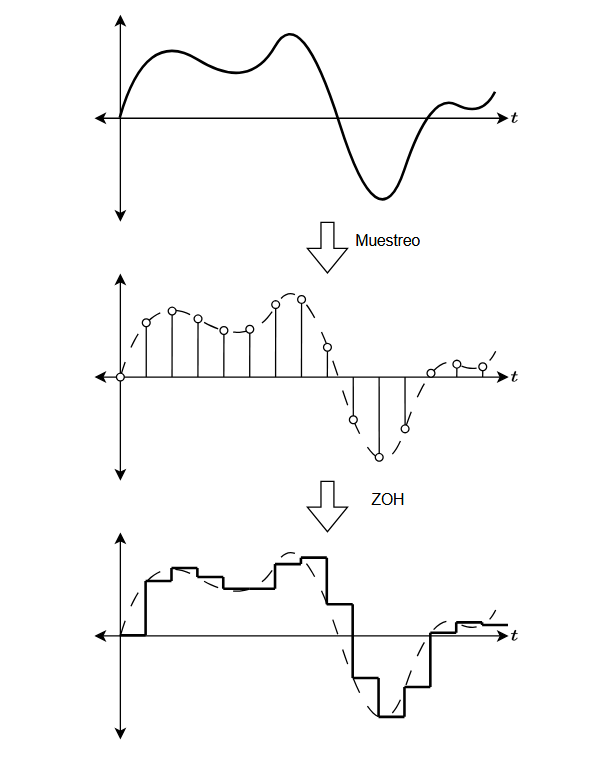
\includegraphics[width=0.6\textwidth]{Auxiliar_5_1}
    \caption{Diagrama de bloques del sistema discreto equivalente al sistema continuo, considerando un ZOH.}
    \label{fig:2_5}
\end{figure}
\subsection*{Resolución 2.6}

Obtener la respuesta al impulso de un sistema discreto es análogo a obtenerla para un sistema continuo: dado que $H(z)=Y(z)/U(z)$, y dado que $\mathcal{Z}\{\delta(n)\}=1$, podemos ver que la respuesta al impulso corresponde a la antitransformada de la función de transferencia. Así, basta aplicar $\mathcal{Z}^{-1}$ al resultado obtenido de $\tilde{H}(z)$ para tener la respuesta al impulso. Haciendo esto, tenemos
\begin{align}
h(n)&=\mathcal{Z}^{-1}\{\tilde{H}(z)\}
&=\frac{1}{2\omega_0^{2} l}\left(
\mathcal{Z}^{-1}\!\left\{\frac{z-1}{z-e^{\omega_0 T}}\right\}
+\mathcal{Z}^{-1}\!\left\{\frac{z-1}{z-e^{-\omega_0 T}}\right\}
-2\,\mathcal{Z}^{-1}\{1\}
\right).
\end{align}
Para calcular las antitransformadas, consideremos que se conoce la siguiente propiedad
\begin{equation}
\mathcal{Z}\{x(n+k)\}=z^{k}X(z).
\end{equation}
Si separamos los términos dentro de las antitransformadas, tenemos
\begin{equation}
\frac{z-1}{z-e^{\omega_0 T}}=\frac{z}{z-e^{\omega_0 T}}-\frac{1}{z-e^{\omega_0 T}},
\end{equation}
donde podemos ver que el término de la izquierda ya está en la forma de la exponencial, por lo que no hace falta manipularlo. Para el término de la derecha, si amplificamos tanto el numerador como el denominador por $z$ tenemos
\begin{equation}
\frac{z-1}{z-e^{\omega_0 T}}=\frac{z}{z-e^{\omega_0 T}}-\frac{1}{z-e^{\omega_0 T}},
\quad\Rightarrow\quad
\frac{1}{z-e^{\omega_0 T}}=\frac{1}{z}\cdot\frac{z}{z-e^{\omega_0 T}},
\end{equation}
por lo que podemos ver que el término de la derecha corresponde a una exponencial con un retardo de una unidad. Así, tenemos
\begin{align}
\mathcal{Z}^{-1}\!\left\{\frac{z-1}{z-e^{\omega_0 T}}\right\}
&=\mathcal{Z}^{-1}\!\left\{\frac{z}{z-e^{\omega_0 T}}\right\}
-\mathcal{Z}^{-1}\!\left\{\frac{1}{z}\cdot\frac{z}{z-e^{\omega_0 T}}\right\}\\
&=e^{\omega_0 nT}-e^{\omega_0 (n-1)T}.
\end{align}
Con un procedimiento análogo se puede ver que
\begin{equation}
\mathcal{Z}^{-1}\!\left\{\frac{z-1}{z-e^{-\omega_0 T}}\right\}
=e^{-\omega_0 nT}-e^{-\omega_0 (n-1)T}.
\end{equation}
Finalmente, considerando que $\mathcal{Z}\{\delta(n)\}=1$, tenemos
\begin{equation}
\boxed{\;
h(n)=\frac{1}{2\omega_0^{2} l}
\Big(
e^{\omega_0 nT}-e^{\omega_0 (n-1)T}
+e^{-\omega_0 nT}-e^{-\omega_0 (n-1)T}
-2\,\delta(n)
\Big).}
\end{equation}
\end{solution}
%--------------------------------
\question Considere un sistema LTI de la siguiente forma
\begin{align*}
\mathbf{x}(k+1) &= \begin{pmatrix} -0.5 & 1 & 0 \\ 0 & -0.5 & 0 \\ 0 & 0 & 1.5 \end{pmatrix} \mathbf{x}(k) + \begin{pmatrix} 1 \\ 1 \\ 1 \end{pmatrix} u(k) \\
y(k) &= \begin{pmatrix} 1 & 1 & 0 \end{pmatrix} \mathbf{x}(k).
\end{align*}

\begin{enumerate}
  \item Obtenga la MTE del sistema, y encuentre las funciones base.
  \item Encuentre la respuesta al impulso del sistema.
  \item Determine estabilidad BIBS y BIBO.
  \item Determine controlabilidad y observabilidad del sistema.
\end{enumerate}
%---------------------------
\begin{solution}

\subsection*{Resolución 3.1}

Dado que para nuestro sistema la matriz $A$ tiene forma canónica de Jordan por bloques, la
potencia es rápida de obtener, por lo que la MTE está dada por
\begin{equation}
\Phi(k)=A^{k}=
\begin{pmatrix}
(-0.5)^{k} & k(-0.5)^{k-1} & 0\\
0          & (-0.5)^{k}    & 0\\
0          & 0              & (1.5)^{k}
\end{pmatrix}
=
\begin{pmatrix}
(-0.5)^{k} & k(-0.5)^{k-1} & 0\\
0          & (-0.5)^{k}    & 0\\
0          & 0              & (1.5)^{k}
\end{pmatrix}.
\tag{3}
\end{equation}

Luego, para encontrar las funciones base, debemos tener en mente que estas corresponden a las componentes linealmente independientes de la respuesta a entrada cero. Expresando esta respuesta a entrada cero, considerando que, por ser LTI, la expresión para esta es conocida, tenemos
\begin{equation}
y_{0}(k)=C\,\Phi(k)\,x(0).
\tag{4}
\end{equation}
Si consideramos condiciones iniciales arbitrarias $x_{1},x_{2},x_{3}$, tenemos
\begin{align}
y_{0}(k)
&=\begin{pmatrix}1&1&0\end{pmatrix}
\begin{pmatrix}
(-0.5)^{k} & k(-0.5)^{k-1} & 0\\
0          & (-0.5)^{k}    & 0\\
0          & 0              & (1.5)^{k}
\end{pmatrix}
\begin{pmatrix}x_{1}\\ x_{2}\\ x_{3}\end{pmatrix}
\tag{5}\\[2pt]
&=\begin{pmatrix}(-0.5)^{k} & k(-0.5)^{k-1}+(-0.5)^{k} & 0\end{pmatrix}
\begin{pmatrix}x_{1}\\ x_{2}\\ x_{3}\end{pmatrix}
\tag{6}\\
&=(x_{1}+x_{2})(-0.5)^{k}+x_{2}\,k(-0.5)^{k-1}.
\tag{7}
\end{align}
Como podemos ver, en la respuesta a entrada cero se pueden identificar dos componentes linealmente independientes:
$(-0.5)^{k}$ y $k(-0.5)^{k-1}$ (es importante notar que la segunda componente incluye al término $k$), por lo que las funciones base son
\begin{equation}
\phi(t)=
\begin{pmatrix}
(-0.5)^{k}\\[2pt]
k(-0.5)^{k-1}
\end{pmatrix}.
\tag{8}
\end{equation}

\subsection*{Resolución 3.2}

Dado que el sistema es LTI, la expresión para la respuesta al impulso es conocida, y tiene la forma
\begin{equation}
h(k)=C\,\Phi(k)\,B,
\tag{9}
\end{equation}
donde podemos ver que corresponde a la RENC evaluando $x(0)=B$. Reemplazando los términos, tenemos
\begin{equation}
h(k)=2(-0.5)^{k}+k(-0.5)^{k-1}.
\tag{10}
\end{equation}

Algo importante a tener en mente es que, si bien en la MTE aparece el término $(1.5)^{k}$, correspondiente a una potencia que diverge (dado que el coeficiente tiene valor absoluto mayor a $1$), este no aparece en la respuesta al impulso, lo cual caracteriza la respuesta del sistema ante una entrada arbitraria. Como veremos al analizar la estabilidad, esto tiene implicancias importantes sobre el comportamiento del sistema.

\subsection*{Resolución 3.3}

Dado que sabemos que la estabilidad BIBS es el criterio más fuerte, ya que implica cualquier otro tipo de estabilidad, comencemos por esta. Dado que el sistema es discreto, para que sea BIBS estable se debe cumplir que $\forall \lambda \in \mathrm{eig}(A)$, $|\lambda|\le 1$ si $\lambda$ es un polo singular, o $|\lambda|<1$ si es un polo repetido.

En este caso, los polos del sistema son $\lambda_{1}=\lambda_{2}=-0.5$ y $\lambda_{3}=1.5$, lo cual se puede identificar rápidamente a partir de la forma canónica de Jordan. Como podemos ver, $-0.5$ es un polo repetido y satisface que $|{-0.5}|<1$, pero el tercer polo no cumple la relación, por lo que el sistema es BIBS inestable.

Dado que el sistema es BIBS inestable, debemos analizar la estabilidad BIBO por separado. Para que el sistema sea BIBO estable, se debe cumplir que
\begin{equation}
\sum_{k\ge 0} |h(k)| < \infty.
\tag{11}
\end{equation}
Reemplazando la respuesta al impulso que expresamos anteriormente, tenemos
\begin{equation}
\sum_{k\ge 0} \big| 2(-0.5)^{k}+k(-0.5)^{k-1} \big|.
\tag{12}
\end{equation}
Como podemos ver, ambas potencias convergen cuando $k\to\infty$, por lo que sería directo verificar que la sumatoria converge y, por lo tanto, el sistema es BIBO estable. En el caso de una evaluación, este argumento es suficiente para concluir la estabilidad; sin embargo, por completitud, haremos la demostración rigurosa de que, efectivamente, la serie converge.

Comencemos notando que la desigualdad triangular nos dice que $|x+y|\le |x|+|y|$. Aplicando esto al valor absoluto dentro de la serie, tenemos
\begin{equation}
\sum_{k\ge 0} \big| 2(-0.5)^{k}+k(-0.5)^{k-1} \big|
\le
\underbrace{\sum_{k\ge 0} \big| 2(-0.5)^{k}\big|}_{S_{1}}
+
\underbrace{\sum_{k\ge 0} \big| k(-0.5)^{k-1} \big|}_{S_{2}}.
\tag{13}
\end{equation}

Analicemos cada serie por separado. Para $S_{1}$, vemos que
\begin{equation}
S_{1}=\sum_{k\ge 0} \big|2(-0.5)^{k}\big|
=2\sum_{k\ge 0} (0.5)^{k},
\tag{14}
\end{equation}
correspondiente a una serie geométrica por lo que, evaluando considerando que $|0.5|<1$, tenemos
\begin{equation}
S_{1}=2\,\frac{1}{1-0.5}=4.
\tag{15}
\end{equation}
Para $S_{2}$, considerando que
\begin{equation}
\sum_{k\ge 1} k r^{k} = \frac{r}{(1-r)^{2}}\quad \text{ssi } |r|<1,
\end{equation}
vemos que
\begin{equation}
S_{2}=\frac{0.5}{0.5^{2}},
\tag{16}
\end{equation}
de modo que
\begin{equation}
\sum_{k\ge 0} |h(k)| \le 4 + \frac{2}{0.5^{2}} < \infty,
\tag{18}
\end{equation}
por lo que el sistema es BIBO estable.

Como podemos ver, este es uno de los casos particulares donde, pese a que el sistema es BIBS inestable, sí es BIBO estable. Esto tiene la interpretación de que hay ciertos estados que, pese a divergir en el tiempo, no son visibles en la salida del sistema y, por lo tanto, no hay forma de visualizar esa divergencia en la respuesta.

\subsection*{Resolución 3.4}

Comencemos analizando la controlabilidad del sistema.

El concepto de controlabilidad tiene que ver con la capacidad de modificar cada uno de los estados con la entrada que es alimentada al sistema. Para determinar si el sistema es controlable, utilizaremos la matriz de controlabilidad $\zeta$. En particular, diremos que el sistema es controlable ssi $\zeta$ es de rango completo, donde
\begin{equation}
\zeta=\big( B\;\; AB\;\; A^{2}B\;\; A^{3}B\;\; \cdots\;\; A^{n-1}B \big).
\tag{19}
\end{equation}

Analizando nuestro caso particular, dado que el sistema es de tercer orden tenemos $n=3$, por lo que
\begin{equation}
\zeta=\big( B\;\; AB\;\; A^{2}B \big).
\tag{20}
\end{equation}
Reemplazando, tenemos
\begin{equation}
\zeta=
\begin{pmatrix}
1 & 0.5 & -0.75\\
1 & -0.5 & 0.25\\
1 & 1.5 & 2.25
\end{pmatrix},
\tag{21}
\end{equation}
donde podemos ver que todas las filas y columnas son l.i., por lo que la matriz es de rango completo y el sistema es controlable. Otra forma de verificar que es de rango completo, sin tener que verificar la independencia de las filas o columnas, es considerar la siguiente propiedad: una matriz $M\in\mathbb{M}_{n\times n}$ es de rango completo ssi $|M|\neq 0$. Así, para verificar que el sistema es controlable podemos calcular el determinante de $\zeta$, donde vemos que $|\zeta|=-4\neq 0$, lo cual coincide con lo que habíamos observado.

Ahora, analicemos la observabilidad.

La observabilidad, similar a lo que ocurría con la controlabilidad, tiene que ver con la noción de que todos los estados tengan alguna contribución discernible en la respuesta del sistema y, por lo tanto, que es posible inferir los estados a partir de la salida. Para verificar observabilidad podemos utilizar la matriz de observabilidad $\vartheta$, dada por
\begin{equation}
\vartheta=
\begin{pmatrix}
C\\
CA\\
CA^{2}\\
\vdots\\
CA^{n-1}
\end{pmatrix},
\tag{22}
\end{equation}
donde la observabilidad se tiene ssi $\vartheta$ es de rango completo.

Analizándolo para nuestro caso particular, tenemos
\begin{equation}
\vartheta=
\begin{pmatrix}
1 & 1 & 0\\
-0.5 & 0.5 & 0\\
0.25 & -0.75 & 0
\end{pmatrix},
\tag{23}
\end{equation}
donde podemos ver que una de las columnas es nula, por lo que es linealmente dependiente del resto, lo que haría que $\vartheta$ no sea de rango completo y el sistema no sea observable. Si utilizamos el criterio del determinante, podemos ver también que $|\vartheta|=0$, verificando que no es de rango completo.

El hecho de que las funciones base no incluyan al factor $(1.5)^{k}$, el hecho de que el sistema sea BIBS inestable pero BIBO estable, y el hecho de que el sistema no sea observable, son todos factores que están íntimamente relacionados entre sí: todos ellos son consecuencia del hecho de que uno de los estados no es visible en la salida, por lo que no afecta la respuesta del sistema.

\end{solution}

\end{questions}
\end{document}